\subsection{线性回归\&逻辑回归}
\textbf{$\checkmark$ 2020-09-30}\\
线性回归研究的问题是多个变量中某个变量和其他变量之间存在的线性关系, 相当于用多个变量线性表示某个变量, 某个变量就称为因变量, 其他变量就称为自变量. 用数学语言来描述的话就是这样的: 
$$
y=b + \sum_{i=1}^{n} w_i \cdot x_i 
$$
在n等于1时, 相当于根据数据拟合一条直线; 在n大于1的时候, 就是多元线性回归了, 此时拟合一个平面. 自变量也可以称为特征. 
构建线性回归模型时, 重要的有这几个点: 发现相关性较高的特征, 发现与因变量无关的特征, 得到最后实际使用的n个特征, 对于实值特征的范围进行约束, 对于类别特征的类别进行处理. 其实, 以上这些主要是针对数据的初步分析和预处理. 
得到处理后的数据, 接下来可以通过随机梯度下降的方法得到最优的权重. 在线性回归中常使用的目标函数是均方误差函数. 为了避免模型过拟合, 目标函数中还可以加入正则化项, 对特征权重进行限制. 

其实线性回归模型很像神经络中的一部分———一个激活函数为恒等映射的神经元, 也可以看做一个神经网络模型———一个只有一层的神经网络模型. 

\textbf{逻辑回归 (Logistic regression, LR) }, 也是在线性回归的基础上的一个分类模型. 如果把线性回归看做神经网络单元, 那么把激活函数替换为非线性的激活函数就是LR了. 从数学形式来看, LR是这样的: 
$$
z = b + \sum_{i=1}^{n} w_i \cdot x_i 
$$
$$
\bar{y} = \frac{1}{1 + e^{-z}} = \frac{e^z}{1 + e^z}
$$
针对一个样本$x$, LR模型得到的就是$\bar{y}$, 很明显这是一个0到1之间的值, 即一个概率值, 当对样本进行类别划分后 (划分为0、1) , $\bar{y}$是类别为1的概率. 二分类LR的目标函数定义如下: 
$$
L(w_1,...,w_n) = \prod_{i = 1}^{m} (\bar{y^i} )^{y^i} \cdot ( 1 - \bar{y^i}) ^ {1 - y^i}
$$
其中 $y^i$为样本$\boldsymbol{x^i}$的实际类别, $y^i \in \{0, 1\}$. 显然这是一个关于权重和偏置的最大似然函数, 对其取对数后得到: 
$$
loss = log L = \sum_{i=1}^{m} \left( y^i log (\bar{y^i}) + (1 - y^i) log ( 1 - \bar{y^i}) \right)
$$

很明显, 线性回归和逻辑回归的目标函数是不一样的, 那么\textcolor{red}{\textbf{为什么LR不使用均方误差损失函数呢}}?\textit{1) 理论上LR也是可以使用均方误差损失函数的, 但是均方误差损失在进行SGD时存在一个问题, 当预测值与真实值相差越大时, 参数变化的越小, 训练的越慢 ({\color{red}这个可以通过均方误差损失函数对参数的求导可以看出}); 2) 交叉熵本质上是在衡量真实分布与预测分布之间的距离, 这个可以通过交叉熵与 KL 散度的关系可以导出. 而均方差损失衡量的是欧式空间中两点的距离. 而 LR 的输出是样本属于正样本的概率, 这显然与 MSE 是不相符的.} 上述的对数似然函数也可以叫做交叉熵. 

对于多类别 (例如类别数为$\mathcal{L}$) 的LR, 可以训练$\mathcal{L}$个二分类的LR, 每个LR只输出样本属于某个类别的概率, 最后进行集成得到最终的输出结果. 此时的目标函数则会发生一点变化: 
$$
loss = \sum_{i=1}^{m} \sum_{l=1}^{\mathcal{L}} \mathbbm{1}\{y^i = l\} log \frac{e^{ \boldsymbol{w^l} \cdot \boldsymbol{x^i} } }{ \sum_{j=1}^{\mathbb{L}} e^{ \boldsymbol{w^j} \cdot \boldsymbol{x^i}} }
$$
其中$\boldsymbol{w^l}$是第$l$个LR模型的权重向量 (包括了偏置) . 

\textbf{$\checkmark$ 2021-10-14}\\
使用最小二乘法 (使用均方误差来求解模型) 求解线性回归时, 令$\boldsymbol{X}, \boldsymbol{w}$分别表示数据集和权重向量 (包含了偏置) , 则均方误差: 
$$
E_{\boldsymbol{\hat w}} = (\boldsymbol{y} - \boldsymbol{X} \boldsymbol{\hat w})^T (\boldsymbol{y} - \boldsymbol{X} \boldsymbol{\hat w})
$$

$E_{\boldsymbol{\hat w}}$对$\boldsymbol{\hat w}$求导: 
$$
\frac{\partial E_{\boldsymbol{\hat w}}}{\partial \boldsymbol{\hat w}} = 2 \boldsymbol{X}^T(\boldsymbol{X}\boldsymbol{\hat w} - \boldsymbol{y})
$$

如果$\boldsymbol{X^T X}$是满秩矩阵或正定矩阵 (可逆, 正定矩阵一定满秩, 因为其特征值都是正的) 时, 即可得到$\boldsymbol{\hat w}$的唯一解; 否则, 则可能存在多个解使均方误差最小, 此时可根据的算法的归纳偏好 (学习算法对某种类型的假设的偏好, 什么样的模型更好, 例如拟合曲线时, 存在多条曲线符合要求, 但是一般选择更平滑的) 决定, 如引入正则化. 

\textbf{$\checkmark$ 2021-10-16}\\
\textbf{从广义线性模型到逻辑回归} \\
对于样例$(\boldsymbol{x}, y))$, 当我们用线性模型的预测值逼近$y$时, 就得到了线性回归模型, 也可以用用线性模型来逼近$y$的衍生物, 该衍生物是$y$的函数, 即: 
$$
g(y) = \boldsymbol{w}^T \boldsymbol{x} + b
$$
则有: 
$$
y = g^{-1}(\boldsymbol{w}^T \boldsymbol{x} + b)
$$
此时, 称$g(\cdot)$为联系函数. 当基于线性模型做分类时, 只需要找到一个联系函数, 将线性回归模型的预测值 (\textbf{注意线性回归的预测目标不是类别, 但是要将这个不是类别的值与类别概率联系起来}) 与分类任务的真实标记$y$联系起来, 即找到$g^{-1}$. 在逻辑回归中, 令$g^{-1}(z) = \frac{1}{1 + e ^{-z}}$, 即为对数几率函数, 则: 
$$
y = \frac{1}{1 + e^{-(\boldsymbol{w}^T \boldsymbol{x} + b)}}
$$
其实, 根据上式可以反推出$g$来, 即: 
$$
g(y) = \ln \frac{y}{1 - y} = \boldsymbol{w}^T \boldsymbol{x} + b
$$
其中$g(y) = \ln \frac{y}{1 - y}$就是\textbf{对数几率}. 所以, 可以这样描述逻辑回归: \textbf{用线性回归来拟合真实标记的对数几率}. 

\textbf{$\checkmark$ 2021-10-28}\\
\textbf{线性回归与均方误差}\ \ \ \
由于真实数据通常是存在噪声的, 所以预测值一般是约等于真实值的, 即$\hat{y} = \boldsymbol{w}^T \boldsymbol{x} \approx y$. 用$\epsilon \sim \mathcal{N}(0, \sigma^2)$表示噪声, 则有: 
\begin{align}
	y &= \hat{y} + \epsilon \nonumber \\
	  &= \boldsymbol{w}^T \boldsymbol{x} + \epsilon 	\nonumber
\end{align}
假设对于样本$(\boldsymbol{x}, y)$, $P(y | \boldsymbol{x}, \boldsymbol{w}, \epsilon) \sim \mathcal{N}(\boldsymbol{w}^T \boldsymbol{x}, \sigma^2)$, 即$P(y | \boldsymbol{x}, \boldsymbol{w}, \epsilon) = \frac{1}{\sqrt{2\pi} \sigma} e^{-\frac{(y - \boldsymbol{w}^T \boldsymbol{x})^2}{2 \sigma^2}}$. 目标是求$\boldsymbol{w}$使$P(y | \boldsymbol{x}, \boldsymbol{w}, \epsilon)$最大, 通过极大似然可得: 
\begin{align}
	\boldsymbol{w} &= \mathop{argmax}_{\boldsymbol{w}} P(D | \boldsymbol{x}, \boldsymbol{w}, \epsilon) \nonumber \\
		&= \mathop{argmax}_{\boldsymbol{w}} \prod_{i=1}^N e^{-\frac{(y - \boldsymbol{w}^T \boldsymbol{x})^2}{2 \sigma^2}} \nonumber \nonumber \\
		&= \mathop{argmax}_{\boldsymbol{w}} \prod_{i=1}^N -\frac{(y_i - \boldsymbol{w}^T \boldsymbol{x})^2}{2 \sigma^2} \nonumber \\
		&= \mathop{argmin}_{\boldsymbol{w}} (y_i - \boldsymbol{w}^T \boldsymbol{x}) \nonumber \\
		&= \mathop{argmin}_{\boldsymbol{w}} \sum_{i=1}^N (y_i - \boldsymbol{w}^T \boldsymbol{x})^2  \nonumber
\end{align}
关于这个假设, 可以这样理解: 当给定$\boldsymbol{x}, \boldsymbol{w}, \epsilon$时, 真实值在$\hat{y}$附近摆动 (即均值为$\hat{y}$) , 同时由于存在噪声, 方差与$\epsilon$的方差相同. 

\subsection{感知机}
感知机是 1957 年提出的一种线性二分类算法. 感知机相当于在特征空间中找到一个分类平面, 将样本分成两类. 感知机模型的数学表达:

$$
f(x) = \text{sign}(w \cdot x + b)
$$

\subsection{LDA}
\textbf{$\checkmark$ 2020-10-16}\\
Linear Discriminant Analysis, 线性判别分析. 一种经典的线性学习方法, 因为最早由Fisher提出, 故也称为\textit{Fisher 判别分析}. 

\paragraph{思想}给定训练集, \textbf{设法}将样本点投影到一条直线($\boldsymbol{w}$)上, 使同类别的投影到尽可能接近、异类样本点投影到尽可能原理 (对比学习) . 对新样本点进行分类时, 将其投影到这条直线上, 再根据投影点的位置来确定新样本的类别 (\tbc{red}{HOW?}) , 或者用于数据降维·. 

\paragraph{两个类别的LDA}给定数据集$D = \{(x_i, y_i)\}_{i=1}^{m}$, 其中$x_i \in \mathbb{R}^n, y_i \in \{0, 1\}$, 欲求解的投影直线为$\boldsymbol{w}$. 声明以下变量: 
\begin{itemize}
	\item $X_0, X_1$分别表示0, 1类样本集合
	\item $\boldsymbol{\mu}_i = \frac{1}{|X_i|}\sum_{x_j \in X_i} \boldsymbol{x_j}, i\in\{0, 1\}$分别表示0, 1类样本的均值
	\item $\boldsymbol{\sum}_i = \sum_{x_j \in X_i} (\boldsymbol{x_j} - \boldsymbol{\mu}) (\boldsymbol{x_j} - \boldsymbol{\mu})^T, i\in\{0, 1\}$分别表示0, 1类样本的协方差矩阵
\end{itemize}

若将样本点投影到直线上, 那么两类样本的协方差分别为$\boldsymbol{w}^T \boldsymbol{\sum_i} \boldsymbol{w}$ (先计算样本点投影到直线上的值, 在分类计算投影点的均值, 再计算协方差) . 根据LDA的目标: \textbf{同类样本点投影后的方差尽量小, 异类样本点投影后距离尽量大}. 注意到LDA是线性的, 异类样本之间的距离可以通过类别中心投影后的距离来反映, 即$||\boldsymbol{w}^T\boldsymbol{\mu}_0 - \boldsymbol{w}^T\boldsymbol{\mu}_1||_2^2$, 那么LDA的目标就成了: 
\begin{align}
	J(\boldsymbol{w}) &= \frac{||\boldsymbol{w}^T\boldsymbol{\mu}_0 - \boldsymbol{w}^T\boldsymbol{\mu}_1||_2^2}{\boldsymbol{w}^T \boldsymbol{\sum_0} \boldsymbol{w} + \boldsymbol{w}^T \boldsymbol{\sum_1} \boldsymbol{w}} \nonumber \\
	&= \frac{\left\|\left(\boldsymbol{w}^{\mathrm{T}} \boldsymbol{\mu}_{0}-\boldsymbol{w}^{\mathrm{T}} \boldsymbol{\mu}_{1}\right)^{\mathrm{T}}\right\|_{2}^{2}}{\boldsymbol{w}^{\mathrm{T}}\left(\boldsymbol{\Sigma}_{0}+\boldsymbol{\Sigma}_{1}\right) \boldsymbol{w}} \nonumber
\end{align}
定义类内散度矩阵(withi-class scatter matrix)$\boldsymbol{S}_w = \boldsymbol{\sum}_0 + \boldsymbol{\sum}_1$, 类间散度矩阵(between-class scatter matrix)$\boldsymbol{S}_b = (\boldsymbol{\mu}_0 - \boldsymbol{\mu}_1) (\boldsymbol{\mu}_0 - \boldsymbol{\mu}_1)^T$. 则$J(\boldsymbol{w})$可写成: 
$$
J(\boldsymbol{w}) = \frac{\boldsymbol{w}^{\mathrm{T}} \mathbf{S}_{b} \boldsymbol{w}}{\boldsymbol{w}^{\mathrm{T}} \mathbf{S}_{w} \boldsymbol{w}}
$$
其中, 分子分母都是关于$\boldsymbol{w}$的二次项, $J(\boldsymbol{w})$是关于$\boldsymbol{S}_b, \boldsymbol{S}_w, \boldsymbol{w}$的广义瑞利商. 因此$J(\boldsymbol{w})$的解与$\boldsymbol{w}$的长度无关 (\tbc{red}{参考瑞利商和广义瑞利商}) , 故可令$\boldsymbol{w}^{\mathrm{T}} \mathbf{S}_{w} \boldsymbol{w} = 1$, 则新的目标为: 
\begin{align}
	& \mathop{min} \limits_{\boldsymbol{w}} -\boldsymbol{w}^T\boldsymbol{S}_b\boldsymbol{w} \nonumber\\
	& s.t. \boldsymbol{w}^{\mathrm{T}} \mathbf{S}_{w} \boldsymbol{w} = 1 \nonumber
\end{align}
通过拉格朗日求解, 并对$\boldsymbol{w}$求导并令之等于0可得: $\mathbf{S}_{b} \boldsymbol{w}=\lambda \mathbf{S}_{w} \boldsymbol{w}$. 可以从两个角度来求解: 
\begin{itemize}
	\item 两边左乘$\boldsymbol{S}_w^{-1}$可以得到: $\boldsymbol{S}_w^{-1} \mathbf{S}_{b} \boldsymbol{w}=\lambda  \boldsymbol{w}$, 即$\boldsymbol{w}$为$\boldsymbol{S}_w^{-1} \mathbf{S}_{b}$的特征向量 (广义特征向量) . 可以解出$\boldsymbol{S}_w^{-1} \mathbf{S}_{b}$最大的$k$个特征值对于的特征向量, 组成一个矩阵$\boldsymbol{W}$, 来对$\boldsymbol{x}_i$降维: $\boldsymbol{W}^T \boldsymbol{x}_i$
	
	\item 从另一个角度看, $\mathbf{S}_{b} \boldsymbol{w} = (\boldsymbol{\mu}_0 - \boldsymbol{\mu}_1) (\boldsymbol{\mu}_0 - \boldsymbol{\mu}_1)^T \boldsymbol{w}$与$(\boldsymbol{\mu}_0 - \boldsymbol{\mu}_1)$同向, 则令$\mathbf{S}_{b} \boldsymbol{w} = \alpha (\boldsymbol{\mu}_0 - \boldsymbol{\mu}_1)$, 则$\boldsymbol{w} = \boldsymbol{S}_w^{-1} (\boldsymbol{\mu}_0 - \boldsymbol{\mu}_1)$. 考虑到数值解的稳定性, 通常会对$\boldsymbol{S}_w^{-1}$进行奇异值分解. 用于分类时, 假设各个类别的样本数据符合高斯分布, 这样利用LDA进行投影后, 可以利用极大似然估计计算各个类别投影数据的均值和方差, 进而得到该类别高斯分布的概率密度函数. 当一个新的样本到来后, 我们可以将它投影, 然后将投影后的样本特征分别带入各个类别的高斯分布概率密度函数, 计算它属于这个类别的概率, 最大的概率对应的类别即为预测类别, 参考\href{https://www.cnblogs.com/pinard/p/6244265.html}{这里}
\end{itemize}


\subsection{决策树}
\textbf{$\checkmark$ 2020-10-22}\\
Decision Tree, 是一种基本的分类与回归方法, 基于树形结构来进行决策. 
\paragraph{思想}数据的特征构成了一个特征空间, 基于训练样本对特征空间进行划分, 最终得到若干子空间 (即决策树的叶子节点) , 每个字空间的类别或值由该空间内的样本决定. 决策树的学习过程就是决策树的生成过程, 当然, 这个决策树是指剪枝后的决策树. 

\paragraph{决策树生成}给定数据集$D = \{(x_i, y_i)\_{i=1}^{m}\}$, 其中$x_i \in \mathbb{R}^n$, $y_i \in C$为类别 (分类) 或者数值 (回归) , 其中样本的特征集为$A$, 最终的决策树为$T$. 

\subparagraph{分类决策树}
\begin{myenumerate}
\item 构建根节点$T$
\item 若$D$中所有样本均为同类$c$, 则$T$为单节点树, 并将该结点的类别设为$c$, 返回$T$; 
\item 若$A = \emptyset$, 或者$D$中样本在$A$中各个特征上的取值均相同, 则$T$为单节点树, 将$D$中样本数最大的类$c$作为$T$的类别, 返回$T$; 
\item 根据\textbf{特征选择}的方法, 从$A$中选择一个最优的特征$A_g$作为划分特征; 
\item 若以$A_g$划分的收益小于收益阈值, 则$T$为单节点数, 将$D$中类别数最大的类$C$作为$T$的类别; 
\item 遍历$A_g$的每一个值$a_i$, 按照$A_g = a_i$将$D$划分为若干子集$D_i$; 
\item 分别以$D_i$作为新的训练集, $A - {A_g}$作为新的特征集, 递归调用上述过程, 返回的子树作为$T$的子节点; 
\end{myenumerate}

\tbc{red}{注意: 上述过程中针对的是离散类型的特征, 对于连续类型的特征, 通常是选择最优的切分点, 但与离散特征不同的是, 连续特征在切分之后, 还可以继续使用; 而离散特征通常不会多次使用 ($A - A_g$) , 因为在生成时根据离散特征的每一个值将当前节点上的样本划分成多个子集, 那么子集内的样本在该离散特征上的取值是一样的. 当然, 这也和划分方法有关, 当划分离散特征时将离散特征的取值集合划分成多个不相交的子集, 那么这个离散特征也应该能多次使用; 同理, 若对连续特征的划分采用了离散化的方法则等同于离散特征}. 

分类树中常用的特征选择方法: 
\begin{itemize}
\item 信息增益. 通过比较划分前与划分后数据集的熵来选择特征. $Gain(D, A_g) = H(D) - \sum_{i=1}^{|A_g|} \frac{|D_i|}{|D|} H(D_i)$. 其中$H(\cdot)$表示信息熵, $D_i$表示以$A_g$的取值对$D$进行划分. 很显然, 第一项为划分前数据集的熵\footnote{$0 \leq H(D) \leq \log_2 |C|$, 可以通过朗格朗日来求带约束的最大最小值证明, 熵越小表明纯度越高}, $H(D) = -\sum_{c=1}^{|C|} \frac{|D_c|}{|D|} \log \frac{|D_c|}{|D|}$, 其中$D_c$表示类别为$c$的样本. 当然, 对于$H(D_i)$或$H(D_c)$, 也是使用$C$来计算熵. 信息增益对特征的取值数量敏感, 偏向于选择取值多的特征. 选择使$Gain(D, A_g)$最大的$A_g$来划分, $ID_3$以信息增益来做特征选择的. 
\item 信息增益率. 解决信息增益偏向取值多的特征的问题, $Gain\_ratio(D, A_g) = \frac{Gain(D, A_g)}{H_{A_g}(D)}$. 为了矫正信息增益的问题, 信息增益率将信息增益除以了特征$A_g$的固有值(intrinsic value). $H_{A_g}(D) = -\sum_{i=1}^{|A_g|} \frac{|D_i|}{|D|} \log \frac{|D_i|}{|D|}$. 显然, $H_{A_g}(D)$是对$Gain(D, A_g)$的类似于归一化的操作, 取值数越多的特征, 其$H_{A_g}(D)$越大. 选择使$Gain\_ratio(D, A_g)$最大的$A_g$来划分, $C4.5$使用增益率做特则选择. 
\item 基尼指数. $D$的基尼指数为$Gini(D) = \sum_{c}^{C} \sum_{c' \neq c}^{C} p_c p_{c'} = \sum_{c}^{C} p_c (1 - p_c) = 1 - \sum_{c}^{C} p_c^2$, 同样, 基尼指数越小, 纯度越高/不确定性越低. $D$在$A_g$下的基尼指数$Gini(D, A_g) = \sum_{c=1}^{|C|} \frac{|D_c|}{|D|} Gini(D_c)$, 选择\textbf{使$Gini(D, A_g)$最小的特征$A_g$来划分}. $CART$决策树使用基尼指数做特征选择. 
\end{itemize}

\tbc{red}{注意: 以上特征选择方法对连续特征和离散特征都适用, 并不影响$H(\cdot)$的计算, 关键在于是针对分类任务还是回归任务. }

通常, 最终的决策树是经过剪枝生成的. 生成过程中的剪枝 (预估结点划分前后带来的收益, 判断是否继续划分) 称为\textbf{预剪枝}, 生成完整的决策树后再剪枝称为\textbf{后剪枝} (自底向上对非叶子节点进行评估, 是否将以该结点为根节点的子树替换为叶子节点) . 
\begin{itemize}
\item \textbf{预剪枝}. 可以通过设置收益阈值, 或者使用验证集评估划分前后的预测效果来决定是否对结点进行划分 (即是否以该节点为根节点继续划分) . 或者, 该节点内样本是否都属同一类, 节点内样本数量是否小于阈值, 类别分布独立于可用特征 (即划分到该节点时的$A$) , 树是否达到了一定高度. 
\item \textbf{后剪枝}. 递归地从最后一个内部节点开始评估, 评估该节点剪枝前后决策树在验证集上的表现, 如果没有提高则不对该内部节点剪枝, 否则将其收缩为叶子节点, 在新的决策树上继续简直. 
\end{itemize}

\subparagraph{回归决策树}显然, 回归决策树是用来解决回归任务的, 预测连续的数值. 回归决策树的生成过程与分类决策树很相似, 但是有一个比较大的不同: \textbf{回归树通常是二叉树}. 回归树也是对特征空间进行划分, 每次划分时, 选择一个最优的特征及该特征的最优切分点, 根据切分点将样本集划分为两个子集, 继续分别在两个子集上进行划分 (\textbf{在两个子集上依然会使用上一层使用过的特征, 但是由于子集中该特征的值都小于某个阈值, 所以虽然可能会多次使用一个特征, 但是每次的切分点不一样}) , 最终每个子空间上有一个回归值. 

\subparagraph{常见问题}
\begin{myenumerate}
\item 生成决策树过程中, 如何处理某个特征值缺失的样本?可以将该特征上缺失值的样本同时划入到所有子结点中, 或者专门增加一个子节点, 对应特征值缺失的样本. 
\item 
\end{myenumerate}


\subsection{决策树之我见}
决策树算法作为一种树形结构的算法, 树中的内部节点代表对样本的一次判断, 叶子结点表示了对应的预测值. 内部节点的判断可以视作对特征空间的一次次划分. 决策树算法的两个需要学习的地方: \textbf{树形结构}, \textbf{叶子结点对应的值}. 树形结构由内部节点确定, 即按照什么规则对特征空间划分; 叶子结点的值则由其对应的特征空间来得到. 这两个部分通过数据集学习得到. 

一个一般化的决策树学习过程: 
\begin{myenumerate}
	\item 给定一个数据集, 由很多歌样本组成, 每个样本由多个属性组成; 
	\item 为数据集初始化一个结点; 
	\item 按照停\textbf{止准则}判断是否对该结点进行划分. 
	\item 如果不划分, 则该节点作为叶子节点, 并按照指定的策略\textbf{确定叶子节点的值}, 并转到下一个待划分的节点直至没有节点需要划分; 
	\item 如果需要划分, 则从 4 开始继续流程; 
	\item 按照一定的准则从\textbf{候选的}属性集中选择一个属性; 
	\item 按照选择的属性, 对当前结点上的样本进行\textbf{划分}; 
	\item 划分后, 原数据集变成多个小的数据集; 
	\item 遍历每个子数据集, 跳转到 1 执行, 当前节点作为子数据集的父节点. 
\end{myenumerate}


从上面可以看到有一些重点: 1) 停止准则; 2)确定叶子结点的值; 3)候选属性; 4)划分.

\subsubsection{停止准则}
这个比较好理解, 也就是我们确定一个结点是否继续分裂的依据, 当然也决定了整棵决策树是否继续生长. 

!!对于一个结点来说: 1) 如果其划分后的收益过小 (小于阈值) , 我们可以不对其进行划分; 2) 如果改结点内的样本的目标值方差 (连续值) 很小或者纯度很高 (类别) , 也没必要继续划分了; 3) 如果结点上的样本数太少了也没必要划分了; 4) 其他要求. 

对于一棵树来说: 1) 如果树的高度超过了阈值就不划分了; 2) 叶子结点超过一定数量就不划分了; 3) 其他要求.

停止准则作为结束划分的标准, 其实也起到了对树的复杂度进行约束的作用. 

\subsubsection{确定叶子结点的值}
决策树既然是做决策, 那么肯定是要有输出的, 叶子结点的值就是输出. 在给定树结构后, 每个叶子结点对应特征空间中的一块区域, 我们需要为每块区域指定一个输出. 这块特征空间可以看成 n 维空间中的一块区域 $\Omega$, 假设我们通过 $f: \Omega \longmapsto \mathcal{T}$, 其中 $\mathcal{T}$ 是我们的目标空间. 由于在该节点上一些样本, 我们可以把这些样本看作是对 $f$ 的一个采样, 即由这些样本来确定 $\Omega$ 的输出. 对于回归任务来说, $\mathcal{T}$ 可以是实数集 (或其子集) , 可以取均值作为输出; 对于分类任务, 则为离散的空间, 可以以投票的方式来确定输出, 投票又可以是朴素的投票, 或者带权的投票. 


\subsubsection{候选属性}
即那些属性可以用来进行划分. 其实这是一个比较小的细节, 且与具体的划分方法有关. 

对于一个类别属性: 1) 按照该属性的取值进行划分, 得到的子集在该属性上的取值都是一样的, 该特征也就没有必要出现在候选属性里; 2) 将该属性的取值划分为多个不重叠且不为空的子集, 那么该属性还是可以继续用的.

对于连续类型的属性: 1) 如果对值域进行二分, 那么该属性还是可以继续用的, 且这也是一般做法; 2) 如果对该属性进行离散化, 那么将等同于类别属性.

\subsubsection{划分}
重头戏来了. 划分应该是决策树生成过程中最多的操作了吧. 划分时的主要工作包括: 选择最优的属性、在该属性上对数据集进行划分. 

\paragraph{选择哪个属性?}
现有的一些准则有: 信息增益、信息增益率、基尼指数、基于误差的. 其中前三种主要用在分类任务中, 基于误差 (损失) 的主要用在回归中. 当然处了分类、回归, 还有\textbf{排序任务}, 这个暂时还不太了解. 

\subparagraph{分类任务}
对于类别型的属性, 可以通过计算候选集中的每个属性来得到该属性在指定准则下的值, 选择最优的即可. 对于连续型的属性, 通常选取一个阈值将数据集二分后在指定准则下计算收益. 

\subparagraph{回归任务}
对于类别属性, 可以计算按照这个属性进行划分后, 每个子集的误差. 对于连续型属性, 通常会选择多个\textbf{切分点}, 按照切分点将数据集分成多个子集 (可能是多叉树或二叉树) , 对每个子集计算误差. 可以看到其实是一样的, 划分多个子集后计算误差. 注意这个误差, 以均方误差为例, 需要计算划分后对应的特征空间的输出 (并不是最终的叶子结点的输出) , 再与每个样本的目标值计算误差. 

\paragraph{对数据集划分}
这个主要属性的类型. 

对于离散型属性, 可以按照该属性的取值将数据集划分多个子集, 即多叉树, 也可以将属性的取值划分成两个不相交的子集, 即二叉树. 

对于连续型属性, 可以对其进行离散化作为离散型属性处理, 也可以选择切分点, 做二分处理. 

\paragraph{题外话}
在一些开源的工具中, 如 xgboost, 其是以 CART 作为弱学习器. 而原始的 CART 是无法处理类型属性的. 因此早期的 xgboost 也是无法处理类别特征的, 因此通常会对类别特征进行 one-hot 展开, 当作连续特征处理. 虽然也算一种解决办法, 但是 one-hot 处理类别特征又一些比较明显的问题: 
\begin{myitemize}
	\item 当类别的基数很大时, 会消耗更多的空间和时间; 
	
	\item one-hot 处理后, 节点分裂时, 相当于使用了 one-vs-rest 的方式进行划分. 这有什么问题呢?如果该特征的该值上的样本很少时会产生且切分不均衡的问题. 而且使得分割后的特征空间很零碎, 在这样的空间上的出的预测值不准确, 相当于空间太小, 统计上可信度不高; 
\end{myitemize}

但是在后续的更新中, xgboost 开始原生支持类别特征了, 不需要 one-hot 处理类别特征了. 对于一个基数为 $n$ 的类别特征, 将其划分为两个子集的划分方法有 $C_n^1 + C_n^2 + \cdots +C_n^{n-1}$ 种, 如果遍历的话, 复杂度为 $O(2^n)$, 显然这是不可接受的. 一种方案, 以二分类为例: 按照类别特征的取值将数据集进行划分, 统计每个子集里样本的样本的目标值的均值 (即将标签相加后求除以子集里的样本数) , 按照均值对这些取值排序后寻找分割点. 可以证明在分类任务和回归任务中, 这样做能达到最优效果. 

\subsection{GBDT}

\subsection{随机森林}
听名字就知道咋回事了: 很多棵决策树组成的学习器, 不过随机俩字何解呢? RF 的基本流程:
\begin{itemize}
	\item 给定数据集 $\mathcal{D}  = \{(x_i, y_i)\}_{i=1}^n$, 设置停止条件;
	
	\item 按照有放回抽样选择 $n$ 个样本, 作为当前决策树的训练集, 在每个结点分裂时随机选择 $p$ 个特征作为候选的分裂特征, 学习一棵决策树. 由于是放回抽样, 每个样本被选中的概率约等于 63\%, 因此每个样本会作为 37\% 的决策树的\textbf{袋外样本}. 对于每个样本 $x$, 用未使用 $x$ 训练的决策树对其进行预测, 以此计算每一个样本的预测值, 这样既可获得整个数据集上的袋外误差 (out-of-bag error);
	
	\item 重复直至达到终止条件;
\end{itemize}

显然, RF 的随机来自于样本抽样和特征抽样, 为什么要做这个呢? 尽量降低每棵树之间的相关性. Bagging 的集成学习一个关键之处就在于构建大量不同的学习器.

RF 特点: 1) 能够处理高维数据, 即在分裂时选择一个特征子集; 2) 随机性使得 RF 有较强的鲁棒性; 3) 树的学习是可并行的; 4) 类别不平衡, 缺失值较多对模型的影响相对较小. 因为会对样本进行抽样, 可以一定程度上降低类别不平衡的影响; 5) 也因为随机性, 不好控制学习过程中使用的特征集合; 6) 数据集较小时, 随机的作用较小.

\subsection{GMM}
Gaussian Mixture Model, 高斯混合模型. 

\subsection{Kmeans}
一种基于划分的聚类算法. Kmeans 通过最小化样本到质心的距离来对样本点进行划分. Kmeans 的流程:
\begin{enumerate}
	\item \textbf{初始化质心}. 初始化 $K$ 给质心, 每个质心代表一个簇;
	
	\item \textbf{计算距离, 分配到簇}. 计算每个样本到各个质心的距离, 将其分配到离其最近的簇;
	
	\item \textbf{更新质心}. 更新每个簇的质心;
	
	\item 判断是否收敛, 是的话则结束, 否则重复上述两步;
\end{enumerate}

可以看见 Kmeans 还是很简单的, 主要是计算样本点到质心的距离并进行分配. 因此该算法的计算量也主要集中在距离的计算上, 如果数据的维度很高时则会比较耗时, 因此在 Kmeans 前通常会进行降维.

影响 Kmeans 聚类效果的关键: \textbf{$K$ 的选择}, \textbf{初始质心的选取}. 一共要聚类成多少簇这是个要预先设置的超参数, $K$ 的大小直接决定了聚类的效果, 常用的方法:
\begin{itemize}
	\item 设定一个聚类效果好坏的准则, 例如所有样本的对应簇的距离和. 计算随着 $K$ 增大时准则的变化情况. 当 $K$ 小于真实簇数时, $K$ 的增加会对效果产生很大的影响, 准则的值变化明显, 当 $K$ 大于真实簇数时, $K$ 的增加不会对准则产生很大影响. 因此可以画出准则与 $K$ 的关系图, 找到那个分结点作为 $K$ 的值. 这个方法也叫 \textbf{手肘法}.
	
	\item 轮廓系数. 轮廓系数定义为: 每个样本都可以计算一个轮廓系数, 
	$$
	S = \frac{b - a}{max(a, b)}
	$$
	$a$ 表示样本到同簇样本的平均距离, $b$ 表示样本到 (所在簇之外的) 最近簇中所有样本的平均距离. 计算每一个样本的轮廓系数然后求平均作为当前聚类效果的一个评估. 显然轮廓系数越大越好. 
	
	\item \href{https://scikit-learn.org/stable/modules/clustering.html#calinski-harabasz-index}{CH 指标}. 这个指标通过类间方差与类内方差的比来衡量聚类的效果.
\end{itemize} 

其实通过上述方法也可以看出来, 选择 $K$ 的方法基本就是: 定义一个评估聚类效果的准则, 然后尝试不同 $K$ 进行聚类并进行评估, 选择评估效果最好的那个 $K$.


初始化的方法有:
\begin{itemize}
	\item 随机初始化. 很简单粗暴, 直接在数据集中随机选择 $K$ 个样本作为初始质心;
	
	\item Kmeans++. 基本思想: 先随机选择一个质心, 然后再逐步地选择离已有质心 (这里是计算一个点到一个点集的最短距离, 一般是用其中的最小值表示) 最远的点作为新的质心, 直至得到 $K$ 个质心;
	
	\item 可以在随机选择的基础上做多组实验, 选择其中一组最好的;
	
	\item 通过层次聚类得到 $K$ 个簇, 每个簇中的样本的均值作为质心;
\end{itemize}

Kmeans 的\textbf{特点}: 1) 原理简单, 实现也简单; 2) 需要选择 $K$ 和初始化质心; 3) 对于非凸的数据 (类似于流形) 效果不太好, 可以选用基于密度的算法; 4) 可能会处于局部最优; 5) 对噪音和异常点比较敏感, 因为噪音/异常点的对计算质心时影响很大, 可以选用 \textbf{K-中心点}. 该算法与 Kmeans 很相似, 差别在于簇心的计算方式不一样, 在已知 $K$ 个簇心的条件下, 根据距离对数据集进行划分, 但是确定新的簇心时并不是求簇内样本点的均值, 而是依次遍历簇内每一个点, 计算其到簇内其他点的距离之和, 选择距离和最小的作为新的簇心. 显然, K-中心点中的簇心一定是数据集中的样本, 但计算量明显增大了.

\subsection{Spectral cluster}
谱聚类. 将每个样本视作某个空间中的点. 

参考资料: 
\begin{enumerate}
	\item \href{https://www.cnblogs.com/pinard/p/6221564.htm}{谱聚类原理总结}
\end{enumerate}

\subsection{t-SNE}
t-distributed Stochastic Neighbor Embedding. 一种数据降维的方法. 

参考资料: 
\begin{enumerate}
	\item \href{https://scikit-learn.org/stable/modules/manifold.html#t-distributed-stochastic-neighbor-embedding-t-sne}{sklearn 中关于tSNE的介绍}
	\item \href{https://www.jianshu.com/p/700f017cd330}{tSNE降维原理}
\end{enumerate}

\subsection{变分贝叶斯}
用来近似计算复杂积分, 在这类模型中一般包含三类变量: 观测变量、未知参数、隐变量, 其中位置参数和隐变量统称为不可观测变量. 变分贝叶斯的目的主要有两个: 
\begin{itemize}
	\item 近似估计不可观测变量的后验概率, 以便通过这些变量做出推断
	\item 对于一个特定的模型, 给出观测变量边缘似然函数的下界, 作为模型选择的依据. 一般认为似然概率越高, 模型效果越好
\end{itemize}
通常情况下, 我们会有一组观测数据 (D) , 那么怎么获得不可观测变量 (Z) ) 的后验概率P(Z | D)呢?

通常不可观测变量的后验概率是很复杂的, 难以直接计算之, 但我们可以先假设一个分布Q(Z)与P(Z|D)是近似的. 对于衡量两个分布的差异, 可以使用KL散度, 即: KL(Q(Z) | P(Z|D)) . 

$$
\begin{equation}\nonumber
	\begin{aligned}
		KL(Q(Z) || P(Z|D)) &= \sum_{z \in Z} Q(z) \log \frac{Q(z)}{P(z|D)} \\
		&= \sum_{z \in Z} Q(z) \log \frac{Q(z) P(D) )}{P(z, D) } \\	
		&= \sum_{z \in Z} Q(z) ( \log \frac{Q(z)}{P(z|D)} + \log P(D) ) \\
		&= \log P(D) + ( \sum_{z \in Z} Q(z) \log \frac{Q(z)}{P(z, D)}) ) 
	\end{aligned}
\end{equation}
$$

显然只要最小化KL散度即可, 因为$\log P(D)$是一个常数, 所以只要最小化$\sum_{z \in Z} Q(z) \log \frac{Q(z)}{P(z, D)})$即可. 将$\sum_{z \in Z} Q(z) \log \frac{Q(z)}{P(z, D)})$记为$\mathcal{L}$, 则$\log P(D) = -\mathcal{L} + KL(Q || P)$. 显然KL散度一定是非零的, 所以$\log P(D)$的下界就是$-\mathcal{L}$. 


\subsection{自编码器/变分自编码器}
自动编码器是一种无监督的神经网络, 用于学习输入数据的低维表示, 并能够根据低维表示重建输入数据, 也是一种将为的手段. 

变分自动编码 (Variational Auto Encoder) 器运用了变分贝叶斯的思想, 也继承了自动编码器的结构, 但是存在一定的差别. 在VAE中, 默认将输入数据的低维表示 (即隐变量) 服从某个分布, 一般认为服从正态分布. 在encoder阶段学习到隐表示的分布 --- 通常是学习到假定分布的参数, 得到分布后就从该分布中进行采样得到隐表示; decoder时, 则将隐表示输入到decoder中. 

参考资料: 
\begin{itemize}
	\item \href{https://www.cnblogs.com/kexinxin/p/9858525.html}{变分自动编码器}
	\item \href{https://github.com/cdoersch/vae_tutorial}{vae\_tutorial}
\end{itemize}

\subsection{SVM}
一种二分类模型, 定义在特征空间上的间隔最大化的线性分类器, 通过间隔最大化找到支持向量来完成算法的学习. 

给定数据集: $D = \{(x_1, y_1), (x_2, y_2), ..., (x_N, y_N)\}, x_i \in \mathcal{X} = \mathbb{R}^n, y_i \in \mathcal{Y} = \{-1, +1\}, i = 1, 2, ..., N$. 目的是找到最优的超平面$w^T x + b = 0$对$D$进行划分. 

\paragraph{间隔最大化}如果一个\textbf{超平面能够正确划分所有样本}, 则有: 
$$
\begin{cases}
	{w}^{\mathrm{T}} {x}_{i}+b > 0, & y_{i}=+1 \\ 
	{w}^{\mathrm{T}} {x}_{i}+b < 0, & y_{i}=-1
\end{cases}
$$ 
从上式可以得出, 分别存在$0 < \alpha = min(\{w^T x_i + b | y_i = +1\}), 0 > \beta = max(\{w^T x_i + b | y_i = -1\})$使, 
$$
\begin{cases}
	{w}^{\mathrm{T}} {x}_{i}+b \geqslant \alpha, & y_{i}=+1 \\ 
	{w}^{\mathrm{T}} {x}_{i}+b \leqslant \beta, & y_{i}=-1
\end{cases}
$$
对$(w, b)$进行缩放, 令$w = \frac{w}{min(|\alpha|, |\beta|)}, b = \frac{b}{min(|\alpha|, |\beta|)} $, 则有: 
$$
\begin{cases}
	{w}^{\mathrm{T}} {x}_{i}+b \geqslant +1, & y_{i}=+1 \\ 
	{w}^{\mathrm{T}} {x}_{i}+b \leqslant -1, & y_{i}=-1
\end{cases}
$$
其中, 使上式等号成立的样本点为\textbf{支持向量}. 

由于划分超平面有很多, 直觉上, 我们希望划分超平面能够尽可能位于两类样本中间, 即间隔两类样本最大超平面, SVM中是这样定义间隔的: \textbf{两个异类支持向量到超平面的距离之和}, 即: 
$$
\gamma = \frac{2}{||w||}
$$
$\gamma$就是\textbf{\textcolor{red}{间隔}}, 间隔最大化的物理意义: 
\begin{itemize}
	\item 间隔越大, 表示分类的置信度越大, 对hard样本也能够有较高的分类置信度
	\item 间隔越大, 泛化性能越好
	\item 间隔越大, 对噪声的鲁棒性更强
\end{itemize}


\paragraph{间隔最大化的最优化目标}
\begin{align}
	\mathop{max}_{w, b}&\quad \frac{2}{||w||} \nonumber \\
	s.t.&\quad y_i(w^T x_i + b) \geqslant 1, i = 1, 2, ..., N \nonumber
\end{align}
对上式进行简单的转化, 可得: 
\begin{align}
	\mathop{min}_{w, b}&\quad \frac{1}{2}||w||^2 \nonumber \\
	s.t.&\quad y_i(w^T x_i + b) \geqslant 1, i = 1, 2, ..., N \nonumber
\end{align}
优化目标中的约束, 就是我们的期望: 超平面能够将所有样本正确分类, 这也是我们的一个假设, \textcolor{red}{\textbf{数据集$D$是线性可分的!}}. 但很不幸, 很多情况$D$都不是线性可分的!

\textbf{$\checkmark$ 2021-11-18}\\
\paragraph{SVM优化目标推导的另一形式}
给定分离超平面$w^T x + b = 0$, $\forall x_i \in D$, $x_i$与分离平面的距离$d(w, b; x_i) = |w^T x_i + b|$, 则$D$与分离超平面的距离为其中的最小者, 及$d(w, b; D) = \mathop{min}_{x_i} |w^T x_i +b|$, 因为$w, b$按比例变化后分离超平面并不变但会带来距离的变化, 故令$d(w, b; D) = \mathop{min}_{x_i} \frac{|w^T x_i + b|}{||w||}$. 若分离超平面能对所有样本正确分类, 则会有$y_i ( w^T x_i + b ) \geq 0$, 且显然$y_i ( w^T x_i + b ) \geq \mathop{min}_{x_i} |w^T x_i + b|$, 由于可以改变$w, b$来控制距离, 则令$\mathop{min}_{x_i} |w^T x_i + b| = 1$, 则得到了$y_i ( w^T x_i + b ) \geq 1,\ d(w, b; D) = \mathop{min}_{x_i} \frac{1}{||w||}$. 但是为了让$d(w, b; D)$尽量大 (以保证置信度和鲁棒性) , 因此, 优化目标为: 
\begin{align}
	\mathop{max}_{w, b}&\quad \frac{2}{||w||} \nonumber \\
	s.t.&\quad y_i(w^T x_i + b) \geqslant 1, i = 1, 2, ..., N \nonumber
\end{align}

\textbf{$\checkmark$ 2021-11-18}\\
\paragraph{SVM优化目标推导的再一形式}
由上述可知, 显然有$y_i ( w^T x_i + b ) \geq 1$, 则分离超平面与两类样本的距离为: 
\begin{align}
	d(w, b) &= \mathop{min}_{x_i, y_i=-1} d(w, b; x_i) + \mathop{min}_{x_i, y_i=+1} d(w, b; x_i) \nonumber \\
			&= 	\mathop{min}_{x_i, y_i=-1} \frac{|w^T x_i + b|}{||w||} + \mathop{min}_{x_i, y_i=+1} \frac{|w^T x_i + b|}{||w||} \nonumber \\
			&= \frac{1}{||w||} ( \mathop{min}_{x_i, y_i=-1} |w^T x_i + b| + \mathop{min}_{x_i, y_i=+1} |w^T x_i + b|) \nonumber \\
			&= \frac{2}{||w||}
\end{align}
后续就不必多言了. 



\paragraph{线性可分SVM的求解}
可以应用拉格朗日对偶性来求解, 将线性可分得SVM最优化问题看作原始问题, 通过求解对偶问题来求解原始问题. 则原始问题为: 
\begin{align}
	\mathop{min}_{w, b}&\quad \frac{1}{2}||w||^2 \nonumber \\
	s.t.&\quad 1 - y_i(w^T x_i + b) \leq 0, i = 1, 2, ..., N \nonumber
\end{align}
转换拉格朗日函数: 
$$
L(w, b, \alpha) = \frac{1}{ 2}  ||w||^2 + \sum_{i=1}^{N} \alpha_i (1  - y_i(w^T x_i + b))
$$
根据拉格朗日对偶性, 原始问题的对偶问题是极大极小问题: 
$$
\mathop{max}_{\alpha} \mathop{min}_{w, b} L(w, b, \alpha)
$$
那么求解过程可以分为: 
\begin{myenumerate}
	\item 固定$\alpha$, 求$\mathop{min}_{w, b} L(w, b, \alpha)$. 这个通过求偏导并令其等于0, 可得: 
	\begin{align}
		w &= \sum_{i=1}^N \alpha_i y_i x_i	\nonumber \\
		&\sum_{i=1}^N \alpha_i y_i = 0 \nonumber
	\end{align}
	
	\item 将$w, b$用$\alpha$相关的式子表示, 求$\mathop{min}_{w, b} L(w, b, \alpha)$对$\alpha$的极大. 代入$L$后得到的: 
	$$
	L(w, b, \alpha) = -\frac{1}{2} \sum_{i=1}^N \sum_{j=1}^{N} \alpha_i \alpha_j y_i y_j (x_i \cdot x_j) + \sum_{i=1}^N \alpha_i
	$$	
	则对偶问题成了 (加了个负号, 转换成了$min$) : 
	\begin{align}
		\mathop{min}_{\alpha}\quad &\frac{1}{2} \sum_{i=1}^N \sum_{j=1}^{N} \alpha_i \alpha_j y_i y_j (x_i \cdot x_j) - \sum_{i=1}^N \alpha_i \nonumber \\
		s.t.\quad &\sum_{i=1}^N \alpha_i y_i = 0 \nonumber \\
				  &0 \leq \alpha_i \leq C, i = 1, 2, ..., N \nonumber
	\end{align}
	原始问题满足相关的条件, 故原始问题的最优解$w^*, b^*$可以通过对偶问题的最优解$\alpha^*$来得到. 先假设已经解得了$\alpha^*$, 则显然有: 
	$$
	w^* = \sum_{i=1}^N \alpha_i^* y_i x_i
	$$
	那么$b$呢?回忆KKT条件\ref{kkt}, 有$\alpha_i^* (1 - y_i(w^* x_i + b^*)) = 0$, 因为$\alpha \neq 0$, 故肯定存在某个分量 $\alpha_j^* \neq 0$, 则: 
	\begin{align}
		&1 - y_j(w^* x_j + b^*) = 0 \nonumber \\
		&\mathop{\Longrightarrow}_{\times y_j} y_j - y_j^2 (w^* x_j + b^*) = 0 \nonumber \\
		&\mathop{\Longrightarrow}_{rep.\  w^*} y_j - 1 \cdot (\sum_{i=1}^N \alpha_i^* y_i x_i x_j + b^*) = 0 \nonumber \\
		&\Longrightarrow b^* = y_j - \sum_{i=1}^N \alpha_i^* y_i (x_i \cdot x_j) \nonumber 
	\end{align}
	注意$y_j$是$\alpha_j^* \neq 0$所对应的样本的标签, 显然, \textcolor{red}{$(x_j, y_j)$就是那些支持向量}, 同理, \textcolor{red}{在计算$w^*$时起作用的是全部的支持向量}. 
	现在, 任务就是如何求出$\alpha^*$了!	求解$\alpha^*$是另一个优化问题了, 通常使用\textit{Sequential Minimal Optimization, SMO}\ref{smo}求解. 
\end{myenumerate}

至此, 得到了$w^*, b^*$, 分离超平面也就确定了$w^* \cdot x + b^* = 0$, 那么也就可以开始使用SVM了, 分类决策函数: 
$$
f(x) = sign(w^* \cdot x + b^*)
$$

在上述过程中, 是否还记得一个假设: \textbf{\textcolor{red}{数据集$D$是线性可分的!}}这个假设对我们的求解过程有什么影响呢?\textbf{\textcolor{red}{不等式约束}}. 对于线性可分的SVM, 是在\textbf{硬间隔最大化}的基础上构建的. 显然, 现实世界没有那么简单!

\paragraph{线性SVM}
这个时候的数据集$D$, 并不是完全线性可分的, 但是除去数据中的一些异常点后, 剩下的点是线性可分的. 这个时候考虑如何将异常点带来的影响融入到模型中. 

若允许一部分异常点被分错, 即
$$
\begin{cases}
	{w}^{\mathrm{T}} {x}_{i}+b > \alpha_i \leq 0, & y_{i}=+1 \\ 
	{w}^{\mathrm{T}} {x}_{i}+b < \beta_i \geq 0, & y_{i}=-1
\end{cases}
$$ 
这个式子的含义是: 对于异常点, 允许其在超平面的另一边. 经过以下转化: 
\begin{quotation}
	$$
	\begin{cases}
		{w}^{\mathrm{T}} {x}_{i}+b - \alpha_i > 0, & y_{i}=+1 \\ 
		{w}^{\mathrm{T}} {x}_{i}+b - \beta_i < 0, & y_{i}=-1
	\end{cases}
	$$
	存在$u >0, v < 0$, 使得: 
	$$
	\begin{cases}
		{w}^{\mathrm{T}} {x}_{i}+b - \alpha_i \geq u, & y_{i}=+1 \\ 
		{w}^{\mathrm{T}} {x}_{i}+b - \beta_i \leq v, & y_{i}=-1
	\end{cases}
	$$
	经过缩放后 (注意$\alpha_i, \beta_i$也缩放了) , 有: 
	$$
	\begin{cases}
		{w}^{\mathrm{T}} {x}_{i}+b - \alpha_i \geq 1, & y_{i}=+1 \\ 
		{w}^{\mathrm{T}} {x}_{i}+b - \beta_i \leq -1, & y_{i}=-1
	\end{cases}
	$$
	移项, 有
	$$
	\begin{cases}
		{w}^{\mathrm{T}} {x}_{i}+b \geq 1 + \alpha_i, & y_{i}=+1 \\ 
		{w}^{\mathrm{T}} {x}_{i}+b \leq -1 + \beta_i , & y_{i}=-1
	\end{cases}
	$$
	左右两边分别乘对应的$y_i$, 同时令\textcolor{red}{$\alpha_i = -\alpha_i$}, 此时, \textbf{\textcolor{red}{$\alpha_i \geq 0, \beta_i \geq 0$}}, 则有: 
	$$
	\begin{cases}
		y_i( {w}^{\mathrm{T}} {x}_{i}+b ) \geq 1 - \alpha_i, & y_{i}=+1 \\ 
		y_i( {w}^{\mathrm{T}} {x}_{i}+b) \textcolor{red}{\geq} 1 - \beta_i , & y_{i}=-1
	\end{cases}
	$$	
\end{quotation}
针对每个样本$(x_i, y_i)$, 给$\alpha_i, \beta_i$取个新的名字$\xi_i$ (\textbf{松弛变量}) , 则有: 
$$
y_i( {w}^{\mathrm{T}} {x}_{i}+b ) \geq 1 - \xi_i
$$
是否感觉\textbf{\textcolor{red}{又回到了最初的起点}}?

注意, 松弛变量是针对每个样本的, 即每个样本都有一个自己的松弛变量, $1-\xi_i$的物理含义是$x_i$里分离超平面的距离, $\xi_i$就是$x_i$离由距分离超平面为1的同类样本点组成的平面的距离, 所以, \textbf{理所当然的希望$\xi_i$尽量小}, 这也是希望异常点不要太异常. 

因此, 很容易可以得到新的优化目标, 其中$C > 0$是\textbf{惩罚参数}: 
\begin{align}
	\mathop{min}_{w, b, \xi}&\quad \frac{1}{2} ||w||^2 + C \sum_{i=1}^{N} \xi_i \nonumber \\
	s.t.&\quad y_i(w^T x_i + b) \geqslant 1 - \xi_i, i = 1, 2, ..., N \nonumber \\
		&\quad \xi_i \geq 0, i = 1, 2, ..., N \nonumber
\end{align}
该问题的对偶问题为: 
\begin{align}
	\mathop{min}_{\alpha}\quad &\frac{1}{2} \sum_{i=1}^N \sum_{j=1}^{N} \alpha_i \alpha_j y_i y_j (x_i \cdot x_j) - \sum_{i=1}^N \alpha_i \nonumber \\
	s.t.\quad &\sum_{i=1}^N \alpha_i y_i = 0 \nonumber \\
	&0 \leq \alpha_i \leq C, i = 1, 2, ..., N \nonumber
\end{align}
求解这个约束优化问题, 同样利用拉格朗日对偶性, 求解过程与线性可分SVM类似, 不再赘述, 且其解为: 
$$
w^* = \sum_{i=1}^N \alpha_i^* y_i x_i
$$
$$
b = y_j - \sum_{i=1}^N \alpha_i y_i (x_i \cdot x_j)
$$
但有一些不同: \textcolor{red}{\textbf{支持向量}}. 经过类比, 很显然, 线性SVM中的支持向量应满足: $1 - \xi_j = y_j ( w^* x_j + b^* ) $, 即支持向量与分离超平面的距离不一定是1, 而是$1 - \xi_j$. 

\subparagraph{合页损失函数}
SVM希望所有样本尽量满足$y_i( w^T x_i + b ) \geq 1$, 考虑损失函数: 
$$
\mathop{min}_{w, b} \frac{1}{2} ||w||^2 + C \sum_{i=1}^{N} max(0, 1 - y_i (w^T x + b))
$$
定义\textit{hinge-loss} (合页损失) $l_{hinge}(z) = max(0, 1-z)$. $l_{hinge}$不仅要求分类正确, 还要求有较高的置信度 (离分类超平面有一定距离) 时损失才为0. $y_i( w^T x_i + b )$表示$x_i$离超平面的距离, \textbf{当错误分类时, 显然损失大于0; 当正确分类时, 显然有$y_i( w^T x_i + b ) \geq 0$, 但这并不能保证这个样本带来的损失为0, 只有当其处于超平面正确的一侧, 且距离大于1 ($y_i( w^T x_i + b ) \geq 1$) 时损失才为0}. 

令$max(0, 1-y_i (w^T x_i + b)) = \xi_i$, 显然$\xi_i \geq 0$, 且当$1-y_i (w^T x_i + b) > 0$时, $1-y_i (w^T x_i + b) = \xi_i$, 当$1-y_i (w^T x_i + b) \leq 0$时, $\xi_i = 0$, 即: 
$$
1-y_i (w^T x_i + b) \leq \xi_i \Longrightarrow y_i (w^T x_i + b) \geq 1 - \xi_i
$$
所以上述损失函数转化为: 
\begin{align}
	\mathop{min}_{w, b, \xi}&\quad \frac{1}{2} ||w||^2 + C \sum_{i=1}^{N} \xi_i \nonumber \\
	s.t.&\quad y_i(w^T x_i + b) \geqslant 1 - \xi_i, i = 1, 2, ..., N \nonumber \\
	&\quad \xi_i \geq 0, i = 1, 2, ..., N \nonumber
\end{align}
可见, 合页损失等价于一个约束优化问题. 

\paragraph{非线性SVM}
在输入空间中, 不能找到一个超平面对不同的类别进行分类. 如果要用SVM来分类的话, 线性模型的SVM该怎么办呢 --- \textbf{将样本空间映射到一个另一个空间中, 目标空间中的样本点是线性可分的}. 那么利用SVM对于线性不可分的$D$进行分类的问题就成了: 1) 空间映射; 2) 求解SVM相关的优化问题. 

\subparagraph{核技巧}
核技巧就是用来进行空间映射的方法. 数据集$D$的源空间为$\mathcal{X}$, 目标空间为$\mathcal{H}$. 定义$\mathcal{X}$到$\mathcal{H}$的映射: 
$$
\phi (x): \mathcal{X} \rightarrow \mathcal{H}
$$
经过$\phi(\cdot)$的映射后的$D$将变成线性的 (注意不一定是线性可分的) , 则根据线性SVM中的对偶问题可得其目标函数为 (省略了约束条件) : 
$$
\mathop{min}_{\alpha}\quad &\frac{1}{2} \sum_{i=1}^N \sum_{j=1}^{N} \alpha_i \alpha_j y_i y_j (\phi(x_i) \cdot \phi(x_j)) - \sum_{i=1}^N \alpha_i
$$
那么, 如何找到映射函数呢?通常, 并不直接定义映射函数, 而是间接定义一个核函数, 用来表示两个样本点在目标空间中的内积, 
$$
\kappa(x_i, x_j) = \phi(x_i) \cdot \phi(x_j)
$$
因此, 在求解时涉及到的样本点的内积都可以用和函数来代替了. 
\textbf{\textcolor{red}{怎么找核函数呢?}}\ref{pdkf}

\subparagraph{求解非线性SVM}
参考线性SVM中原始问题的对偶问题, 可以写出非线性SVM的对偶问题: 
\begin{align}
	\mathop{min}_{\alpha}\quad &\frac{1}{2} \sum_{i=1}^N \sum_{j=1}^{N} \alpha_i \alpha_j y_i y_j \kappa(x_i, x_j) - \sum_{i=1}^N \alpha_i \nonumber \\
	s.t.\quad &\sum_{i=1}^N \alpha_i y_i = 0 \nonumber \\
	&0 \leq \alpha_i \leq C, i = 1, 2, ..., N \nonumber
\end{align}
此时, 可得其解为: 
$$
w^* = \sum_{i=1}^N \alpha_i^* y_i x_i
$$
$$
b = y_j - \sum_{i=1}^N \alpha_i y_i \kappa(x_i, x_j)
$$
则决策函数可写成: 
$$
f(x) = sign(\sum_{i=1}^N \alpha_i^* y_i \kappa(x_i, x)) + b^*
$$

\paragraph{支持向量回归}
Support Vector Regression, 一种线性的回归模型. 此时, 数据集$D = \{(x_1, y_1), (x_2, y_2), ..., (x_N, y_N)\}, x_i \in \mathbb{R}^n, y_i \in \mathbb{R}$. 要学习的模型为: $f(x) = w^T x + b$. 通过损失函数的角度来引出SVR. 

通常的回归模型采用的是均方误差函数, 只有在预测值与真实值完全一样时损失才为0. SVR假设能够容忍模型有$\epsilon$的误差, 可以定义损失函数: 
$$
l_\epsilon (z) = \begin{cases}0, &|z| \leq z \\ |z| - \epsilon, &others \end{cases}
$$
则SVR转化为: 
$$
\mathop{min}_{w, b} \frac{1}{2} ||w||^2 + C \sum_{i=1}^N l_\epsilon (f(x_i) - y_i) 
$$
类比于合页损失, 在$f(x)$两侧引入不同的松弛变量$\xi_i, \hat{\xi_i}$, 则可将上述目标转化为优化问题: 
\begin{align}
	\mathop{min}_{w, b, \xi, \hat{\xi}}\quad &\frac{1}{2} ||w||^2 + C \sum_{i=1}^{N} (\xi_i + \hat{\xi_i}) \nonumber \\
	s.t.\quad &f(x_i) - y_i \leq \epsilon + \xi_i \nonumber \\
			  &y_i - f(x_i) \leq \epsilon + \hat{\xi_i} \nonumber \\
			  &\xi_i \geq 0, \hat{\xi_i} \geq 0, i = 1, 2, ..., N \nonumber
\end{align}
后续求解与上述类似. 


\subsection{PCA}
全称 Principal component analysis, 即主成分分析. PCA 利用正交变换把由线性相关变量表示的观测数据转换为少数几个线性无关变量表示的数据, 少数的线性无关变量就是主成分. 如果从基的角度来看, 就是将数据在原来的相关的基下的表示, 转化为无关的基下的表示. 

一个简单的流程: 
\begin{enumerate}
	\item 给定数据矩阵 $X \in \mathbb{R}^{m \times n}$, 其中 $m$ 表示特征数, $n$ 表示样本数; 
	
	\item 对 $X$ 去中心化后得到 $\hat{X}$; 
	
	\item 求 $\hat{X} \hat{X}^T$  (相当于 $X$ 的协方差矩阵) 的特征向量, 取特征指最大的前 $k$ 个特征向量组成矩阵 $P \in \mathbb{R}^{k \times m}$. $P$ 就是用于降维的矩阵; 
	
	\item 对 $\hat{X}$ 进行降维: $P \hat{X}$; 
\end{enumerate}


\subsection{metric learning} 
度量学习. 学习如何衡量两个对象之间的相似度/距离. 

\subsection{GBDT 与 XGBoost 的对比}
首先, 两种都是 boosting 方法, 加法模型, 都是迭代地去拟合目标值与现有预测值的残差. 它们之间的区别: 
\begin{itemize}
	\item xgboost 对损失函数进行了二阶展开, 利用了一阶、二阶的信息, 以牛顿法求解参数; GBDT 只用到了一阶导信息; 
	
	\item xgboost 支持自定义代价函数, 只需要提高损失函数的一、二阶导即可; 
	
	\item GBDT 以 CART 作为基分类器, xgboost 除了以树为基分类器, 还可以以线性模型作为基分类器; 
	
	\item xgboost 中加入了正则化项; GBDT中没有; 
	
	\item xgboost 中引入了列抽样和行采样; 
	
	\item xgboost 能够自动学习处缺失值的分裂方向; 
	
	\item xgboost 支持节点级别的并行, 并且支持直方图算法; 
\end{itemize}

\subsection{SMOTE}
SMOTE(Synthetic Minority Over-Sampling Technique) 是一种综合采样人工合成数据算法, 用于解决数据类别不平衡问题, 以 Over-sampling 少数类和 Under-sampling 多数类结合的方式来合成数据. 

SMOTE 以每个样本点的 k 个最近邻样本点为依据, 随机的选择 N 个邻近点, 样本点与邻近点进行差值再乘上一个 [0,1] 范围的阈值, 从而达到合成数据的目的. 这种算法的核心是: 特征空间上邻近的点其特征都是相似的. 它并不是在数据空间上进行采样, 而是在特征空间中进行采样, 所以它的准确率会高于传统的采样方式. 这也是为什么到目前为止 SMOTE 以及其派生的算法仍然是较为主流的采样技术的原因. 

\subsection{LightGBM}
\subsubsection{原理}
LightGBM\cite{guo_nips_2017} 诞生于 NIPS'17. 针对现有 GBDT 实现的一些缺点做了改进, 改进的方向主要是: \textit{efficiency} 和 \textit{scalability}. 现有的实现在分裂结点时, 需要扫所有特征在所有样本上的取值来选择分裂特征和分裂点, 这无疑是非常耗时的. 为了解决这个问题, lgb 中提出了两项技术: \textit{Gradient-based One-Side Sampling} (GOSS) 和 \textit{Exclusive Feature Bundling} (EFB). 前者用于减少参与计算的样本, 后者用于减少参与计算的特征.

\paragraph{GOSS}

\begin{figure}[h]
	\centering
	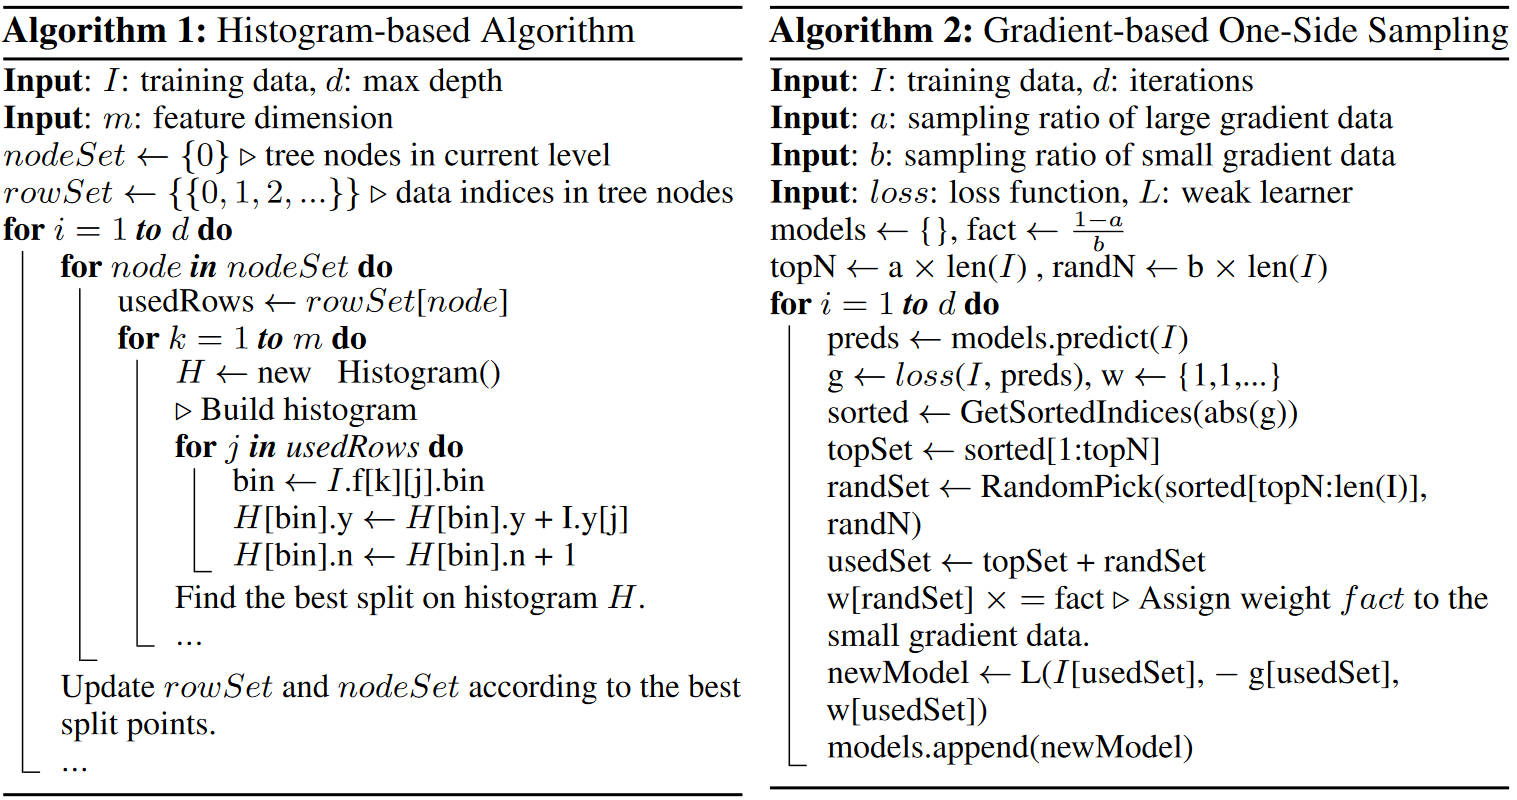
\includegraphics[width=\textwidth]{pics/goss.jpg}
	\caption{Histogram-based Algorithm 和 Gradient-based One-Side Sampling}
	\label{fig:goss}
\end{figure}

基于梯度的单边采样, 在尽量保证效果的基础上过滤掉一部分梯度较小的样本. 因此重点是基于什么来对样本进行过滤? 如果有样本权重, 那么根据权重来采样是可以的, 但很多场景下是没有的. 从 GOSS 的名字也可以看出, lgb 中是\textbf{基于梯度来采样}的. 为什么可以这样呢? lgb 作为 GBDT 的一种实现, 本身也是基于梯度的. 因此如果样本的梯度较小则说明其以及可以被很好分类了, 那么其就是个 \textit{easy sample}, 对于哪些梯度大的则是 \textit{hard sample}. 所以, lgb 中以样本梯度的绝对值作为采样的依据. 但是采样后可能会改变数据的分布, 因此, GOSS 在采样后还有一个缩放的操作. 具体的采样过程其是很简单:
\begin{myitemize}	
	\item 基于已有的模型 (即前面已经训练好的树) 计算每个样本的梯度;
	
	\item 按照梯度绝对值大小对样本进行排序;
	
	\item 取前 $a (\in (0, 1))$ 的数据作为大梯度的样本, 保留下来;
	
	\item 在剩下的 $1-a$ 的样本中随机选择 $b (\in (0, 1))$ 的样本保留下来, 并对这些样本的梯度进行缩放, 乘以 $\frac{1 - a}{b}$;
	
	\item 上两步保留的样本作为这一轮的训练数据;
\end{myitemize}

注意, 根据采样比例计算采样样本数时, 都是相对总样本而言(从 Fig.\ref{fig:goss} 中的 \textit{Gradient-based One-Side Sampling} 可以看出)! 为什么要对小梯度中采样到的样本的梯度进行 $\frac{1 - a}{b}$ 的缩放呢? 

假设小梯度的样本的平均梯度是 $\mu$, 则采样前梯度的总量是 $\text{len}(I) \cdot (1-a) \cdot \mu$, 那么采样后的梯度总量是 $\text{len}(I) \cdot b \cdot \mu$. 为了保持梯度总量不变, 即 $\text{len}(I) \cdot (1-a) \cdot \mu = \text{len}(I) \cdot b \cdot \mu \cdot x$, 显然 $x = \frac{1 - a}{b}$, $x$ 就是缩放系数.

\paragraph{EFB}
互斥特征绑定. 高维的特征大多是很稀疏的, 如果能在牺牲一点点效果的条件下降低特征的维数就可以大大提高性能. 在稀疏的数据中, 存在一些\textbf{互斥的特征}: 这些特征基本上不会同时取非零值. EFB 将这些互斥的特征进行组合作为一个单一的特征, 一次来减少特征的数量. 如何做到呢? EFB 分成两步走: 1) 哪些特征应该被划分到一个 \textit{bundle}; 2) 如何组合 \textit{bundle} 中的特征.

\begin{figure}[h]
	\centering
	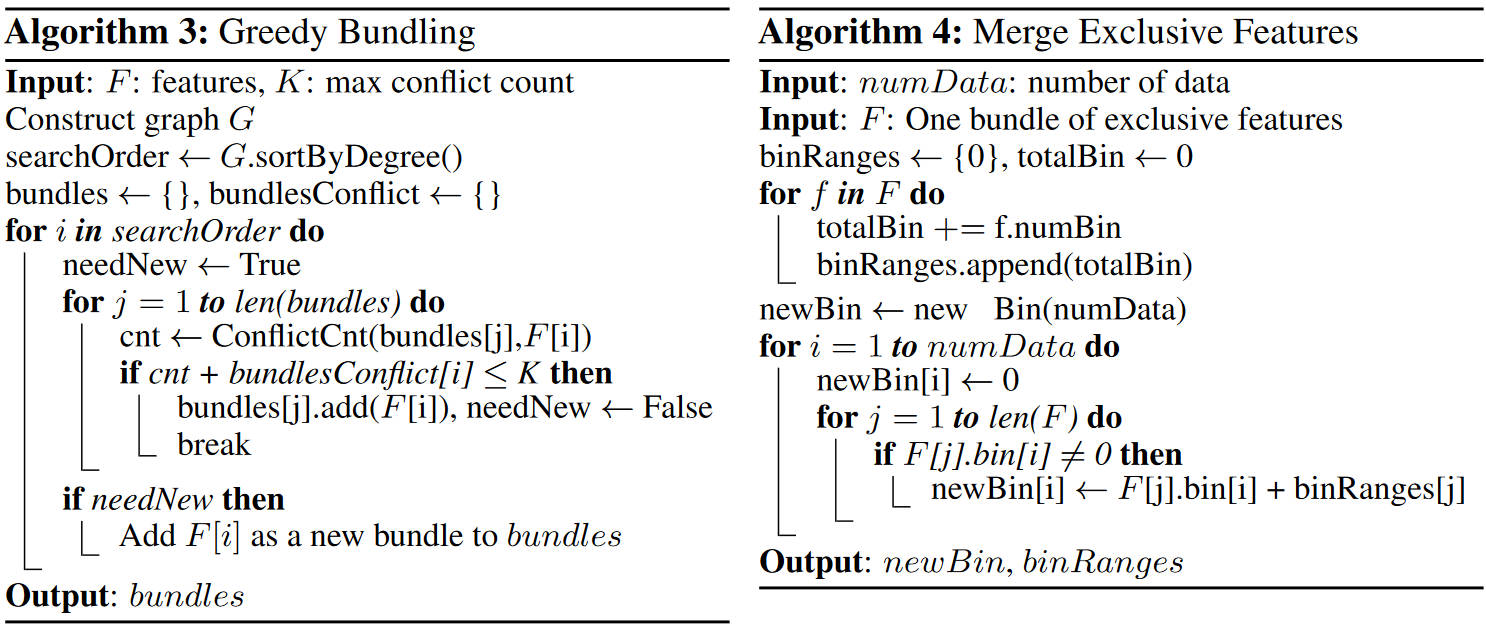
\includegraphics[width=\textwidth]{pics/efb.jpg}
	\caption{EFB 中的两个算法: 构建 \textit{bundle} 和 组合 \textit{bundle} 中的特征}
	\label{fig:efb}
\end{figure}

\subparagraph{Greedy Bundling}
直接对特征进行组合的话将会是一个 NP-hard 的问题, 因此 lgb 将该问题转化为 graph coloring 问题: 将每一个特征视作一个结点, 如果两个特征(结点)不满足互斥的条件则存在边. 再采用贪心的算法来对构建的图进行染色, 最终得到原特征集合的划分, 如 Fig.\ref{fig:efb} 中的 \textit{Greedy Bundling} 所示. 每个 \textit{bundle} 中就是互斥的特征集合. EFB 中并不是严格的互斥, 从算法的伪代码中也可以看到, 冲突次数小于等于 $K$ 是视为互斥的. lgb 中还给出了冲突率和 \textit{accuracy} 的影响的证明. 

\subparagraph{Merge Exclusive Features}
如何把一个 \textit{bundle} 的特征合并为一个特征呢? 一个关键: \textbf{可以从合并后的特征识别处原始特征的值}, 即尽可能降低信息的损失. lgb 中是引入了 \textit{offset} 来帮助区分该值是来源于 \textit{bundle} 中的哪个特征. 例如一个 \textit{bundle} 中的两个特征 $A, B$. 其中 $A$ 的取值范围是 $[0, 10)$, $B$ 的取值范围是 $[0, 20)$. 可以对 $B$ 的取值加上一个值为 10 的 \textit{offset}, 则合并后的特征的取值范围是 $[0, 30)$. 


当然, 除了以上两点, lgb 中还有一些其他改变, 比如改用 \textit{leaf-wise} 的生长策略, 而不是 \textit{level-wise}. 

\textcolor{red}{\textbf{注意}}: 其实关于 lgb 还有一些疑惑, lgb 是否用到了损失函数的二阶导; EFB 之后是怎么进行分裂的.

一些参考资料: \href{https://mp.weixin.qq.com/s/XxFHmxV4_iDq8ksFuZM02w}{LightGBM源码阅读+理论分析(处理特征类别, 缺省值的实现细节)}.

\subsubsection{Core Parameters}
主要参考\href{https://lightgbm.readthedocs.io/en/latest/Parameters.html#}{这里}.
\paragraph{任务相关的参数}
这一部分的参数主要是由你要做什么任务来确定的.
\begin{myitemize}
	\item \mintinline{python}{task} : 指示任务的阶段, 如训练, 预测, 重新拟合等;
	
	\item \mintinline{python}{objective} : 指示要学习的任务的类型, 如回归, 二分类, 多分类, 排序等;
	
	\item \mintinline{python}{boosting} : 使用何种基学习器;
	
	\item \mintinline{python}{num_iterations} : 迭代的次数;
	
	\item \mintinline{python}{num_class} : 类别的数量, 只用在多分类中;
	
	\item \mintinline{python}{learning_rate} : 学习率, 即 xgboost 论文中的 shrinkage rate, 这个参数即控制每一轮学习的幅度, 留一部分学习空间给后来的学习器, 避免一个学习器的效果对目标值起主导作用;
	
	\item \mintinline{python}{tree_learner} : 这个参数控制了并行的粒度;
	
	\item \mintinline{python}{device_type} : 在什么设备上学习, 即 cpu, gpu, cuda, cuda\_exp.
\end{myitemize}

\paragraph{基学习器的参数}
LightGBM 本身也是一种集成学习的方式, 因此关于基学习器也有很多重要的参数, 这些也是调参过程中的主要对象.
\begin{myitemize}
	\item \mintinline{python}{num_leaves} : 树中最大叶子数. 注意与 xgboost 树生长的形式不同, lgb 是按照逐个叶子分裂的. 从树模型的复杂度定义来看, 这个参数影响了模型的复杂度, 因此如果该值过大则容易引发\textbf{过拟合}. 通常, 在相同的叶子数下, 逐层生长的树比逐叶子生长的树要深不少;
	
	\item \mintinline{python}{min_data_in_leaf} : 叶子结点中最少有多少样本. 很显然, 如果这个值设置的比较大, 那么树中的叶子数会比较小, 也能抑制树的生长, 因此可能会引发\textbf{欠拟合};
	
	\item \mintinline{python}{max_depth} : 一棵树的最大高度;
	
	
\end{myitemize}

\paragraph{学习过程中的参数}
这些参数主要是控制学习过程中的行为, 如采样等.
\begin{myitemize}
	\item \mintinline{python}{bagging_freq} : lgb 中有一个 bagging 的概念 (\textbf{\textcolor{red}{还不是很了解}}), 这个参数控制了 bagging 的频率;
	
	\item \mintinline{python}{bagging_fraction} : 如果进行 bagging, 则每次 bagging 时会对数据进行采样, 用采样到的数据进行训练. 这个参数则控制了采样的比例;
	
	\item \mintinline{python}{pos_bagging_fraction / neg_bagging_fraction} : 只在二分类中使用, 控制 bagging 采样时正负样本的比例;
	
	\item \mintinline{python}{min_data_in_leaf} : 树的叶子节点中至少有多少样本. 这个值是根据海森矩阵估计的, 因此在实际中叶子结点中的样本数可能会少于设定的值;
	
	\item \mintinline{python}{feature_fraction} : 列采样的比例. 这个采样是在构建每棵树的时候进行的. 类似的还有 \mintinline{python}{feature_fraction_bynode}, 在每个节点分裂时采样的比例;
	
	
	\item \mintinline{python}{force_col_wise / force_row_wise} : 直方图建立的方式, 逐列或逐行. 这个还不太清楚是啥意思, 可能要看看论文;
	
	\item \mintinline{python}{lambda_l1, lambda_l2} : l1, l2 正则项的系数;
	
	\item 
\end{myitemize}

\paragraph{Dataset 相关的参数}
\begin{myitemize}
	\item \mintinline{python}{max_bin} : 特征分桶时最多可以分多少桶, 也可以通过 \mintinline{python}{max_bin_by_feature} 来指定每个特征最多可以分多少桶;
	
	\item \mintinline{python}{min_data_in_bin} : 一个桶里至少有几个样本;
	
	\item \mintinline{python}{use_missing} : 是否处理缺失值;
	
	\item \mintinline{python}{feature_pre_filtr} : 是否在学习前先过滤一遍特征. lgb 会忽略那些不能用于分裂的特征, 如特征值全都相同的特征, 不能满足 \mintinline{python}{min_data_in_leaf} 的特征;
\end{myitemize}

简单地梳理了一下 LightGBM 的参数, 可以明显地感觉到 lgb 的参数要比 xgb 多, 划分地也更精细.

\subsubsection{调参}
调参, 一般来说是为了获得更好的效果, 但也可以是为了保证一定效果地条件下获得更快的运行速度. 出于不同地目的, 要调整的参数也是不一样的. 这里还是先以效果为目标来介绍调参的过程.
\begin{myenumerate}
	\item 先使用大一些的学习率, 调节 \mintinline{python}{n_iterations}, 即找到大概需要多少轮的增强可以达到较好的效果. 这里先从全局的角度来调. 不涉及每一轮的学习过程中的参数;
	
	\item 接下来调关于每轮学习过程中的参数, 主要是基学习器相关的一些参数. 如 \mintinline[breaklines]{python}{max_depth, num_leaves, min_data_in_leaf, min_data_in_bin, min_sum_hessian_in_leaf, pos_bagging_fraction, neg_bagging_fraction, bagging_freq, bagging_fraction}. 当然, 这几个参数也可以分成几组来调, 可以按照参数的重要性来调节;	
	
	\item 关于正则化项的参数, 如 \mintinline{python}{lambda_l1, lambda_l2, min_gain_to_split, drop_rate} 等;
	
	\item 降低学习率, 并增大迭代的轮数;
	
	\item 可以选择重复上述过程.
\end{myenumerate}
其实, 调参并不能带来大幅的提升, 主要还是看特征工程、模型集成等.

\subsubsection{类别特征的处理}
LightGBM 中引入了对 类别特征的支持, 对于基数较大的类别特征而言, 如果将其展开为 one-hot, 是会有一些坏处的, 例如: 1) 大大增加特征的维数, 空间效率降低; 2) one-hot 展开后, 每个类别上的样本数可能会很少, 分列时是按照 ovr 的形式分裂的, 因为样本过少可能会存在估计不准的情况. lgb 中并不需要将类别特征展开为 one-hot, 可以直接对类别特征进行划分, 按照 many-vs-many 的形式进行划分. 那怎么将一个类别特征的取值划分成两部分呢?

这一过程分成两步:
\begin{enumerate}
	\item 离散特征建立直方图. 众所周知, lgb 中使用了直方图算法来对特征进行分桶, 在这些桶中寻找分裂点. 显然, 也会为离散特征建立直方图, 直方图的每个 \textit{bin} 中保存的是样本的一阶和二阶导数. 当然并不是为每个离散值建立一个 \textit{bin}, 对于那些出现次数过少的离散值则会被过滤掉 (多少算少呢? 这个是可以通过参数 \mintinline{python}{min_data_in_bin} 来指定的);
	
	\item 计算分裂的阈值. 先检查这个时候该特征下 \textit{bin} 的数量, 若其小于一定的数量 (由参数 \mintinline{python}{max_cat_to_onehot} 指定) 时则按照 one-hot 的形式对待, 即 ovr 的形式. 当 \textit{bin} 较多时, 则会根据每个 \textit{bin} 的 \mintinline{python}{sum(gradient) / sum(hessian) + reg} 值来对该特征下的 \textit{bins} 进行排序, 然后遍历每个桶找到最优的切分点.
\end{enumerate}

参考: \href{https://lightgbm.readthedocs.io/en/latest/Features.html#optimal-split-for-categorical-features}{Optimal Split for Categorical Features}.

\subsection{FTRL}
Follow-the-regularized-Leader\cite{hb_ftrl_2010_colt}, 一种在线学习梯度下降优化算法, 能够差生稀疏的解 .

参考资料: \href{https://tech.meituan.com/2016/04/21/online-learning.html}{Online Learning算法理论与实践}, \href{http://vividfree.github.io/%E6%9C%BA%E5%99%A8%E5%AD%A6%E4%B9%A0/2015/12/05/understanding-FTRL-algorithm}{理解 FTRL 算法}.